\subsubsection{\stid{3.14} ForTrilinos}

\paragraph{Overview}

The Exascale Computing Project (ECP) requires the successful transformation and
porting of many Fortran application codes in preparation for ECP platforms. A
significant number of these codes rely upon the scalable solution of linear and
nonlinear equations. The Trilinos Project contains a large and growing
collection of solver capabilities that can utilize next-generation platforms, in
particular scalable multicore, manycore, accelerator and heterogeneous systems.
Since Trilinos is written primarily in C++, its capabilities are not available
to other programming languages. ForTrilinos bridges the gap between the
needs of Fortran app developers and the capabilities of Trilinos. Furthermore,
the technology used to generate the Fortran--C++ bindings in ForTrilinos is
capable of exposing any number of C++ libraries to Fortran exascale app
developers.

ForTrilinos provides a seamless pathway for large and complex Fortran-based
codes to access Trilinos without C/C++ interface code. This access includes
Fortran versions of Kokkos abstractions for code execution and data management.
To provide this functionality, this project developed a Fortran-targeted
extension to the SWIG (Simplified Wrapper and Interface Generator) tool.
Applied to Trilinos, it generates object-oriented Fortran 2003 interface code
that closely mirrors the Trilinos C++ API.

ForTrilinos provides an inversion of control functionality that enables custom
extensions of the Trilinos solvers implemented in downstream Fortran apps.
Although this capability is not yet comprehensive, the goal of this project is
to provide functional and extensible access Trilinos on next-generation
computing systems. Several examples of ForTrilinos are being demonstrated within
Fortran-based ECP codes to help them meet simulation goals and illustrate the
technology to other Fortran-based ECP codes. Additionally, the SWIG technology
underpinning ForTrilinos is being applied to other C++-based ECP ST subprojects
to expose their capabilities to Fortran apps.

\paragraph{Key Challenges}

Developing the interfaces to the C++ libraries that provide access to cutting-edge research, such as Trilinos,  is of significant benefit to Fortran community. However, such interfaces must be well documented, sustainable and extensible, which would require significant amount of resources and investment. This is further complicated by the requirements to support heterogeneous platforms (e.g., GPUs) and inversion-of-control functionality. The manual approach to such interfaces has been shown to be unsustainable as it requires interface developers to have in-depth expertise in  multiple languages and the peculiarities in their interaction on top of the time commitment to update the interfaces with changes in the library.

ForTrilinos addresses both the issue of reducing interface generation cost through investment in tool configuration and usage to make the process as automatic as possible, and the issue of providing the full-featured interface to Trilinos library, including access to manycore, accelerator and heterogeneous solver capabilities in Trilinos.

\paragraph{Solution Strategy}

The ForTrilinos project has two primary thrusts:
\begin{enumerate}
  \item \textbf{SWIG development to support Fortran wrapping:} The new Fortran
    module for SWIG allows for automatic generation of interfaces.
  \item \textbf{Incremental wrapping of selected Trilinos functionality:}
    ForTrilinos provides robust interfaces to selected Trilinos capabilities,
    including distributed data objects, linear and nonlinear solvers.
\end{enumerate}

ForTrilinos started with developing a Fortran module for the Simplified Wrapper Interface Generator (SWIG) utility~\cite{beazley1996swig}. SWIG is used to parse C++ code and generate wrapper code, and was already used for this purpose for several dozen target languages, most notably Python. The project took the approach of adding a Fortran 2003 wrapper generator for SWIG in order to fulfill many of the critical feature requirements for ForTrilinos.

The developed SWIG/Fortran functionality allowed to proceed with automatic generation of Fortran interfaces to selected Trilinos libraries. The work is conducted in phases, with each phase increasing the number of wrapped of Trilinos packages.

The first phase, completed in the first year, developed interfaces for a critical set of features required for solving linear and eigen-problems. The second phase addresses nonlinear solver, including developing automatic approach for inversion-of-control capability. Finally, in the third phase, the challenge of interoperable heterogeneous data passing between Fortran and C++, including GPU data, is addressed, including performance testing.

\paragraph{Recent Progress}

Figure~\ref{fig:fortran_ioc} illustrates a new Inversion-of-Control~(IoC)
implementation in ForTrilinos. The new approach allows Fortran users to define
an operator by using a derived type on the Fortran side, and use Trilinos
algorithms, e.g. Krylov solvers, to solve the linear system with that operator.

\begin{figure}[htb]
    \centering
    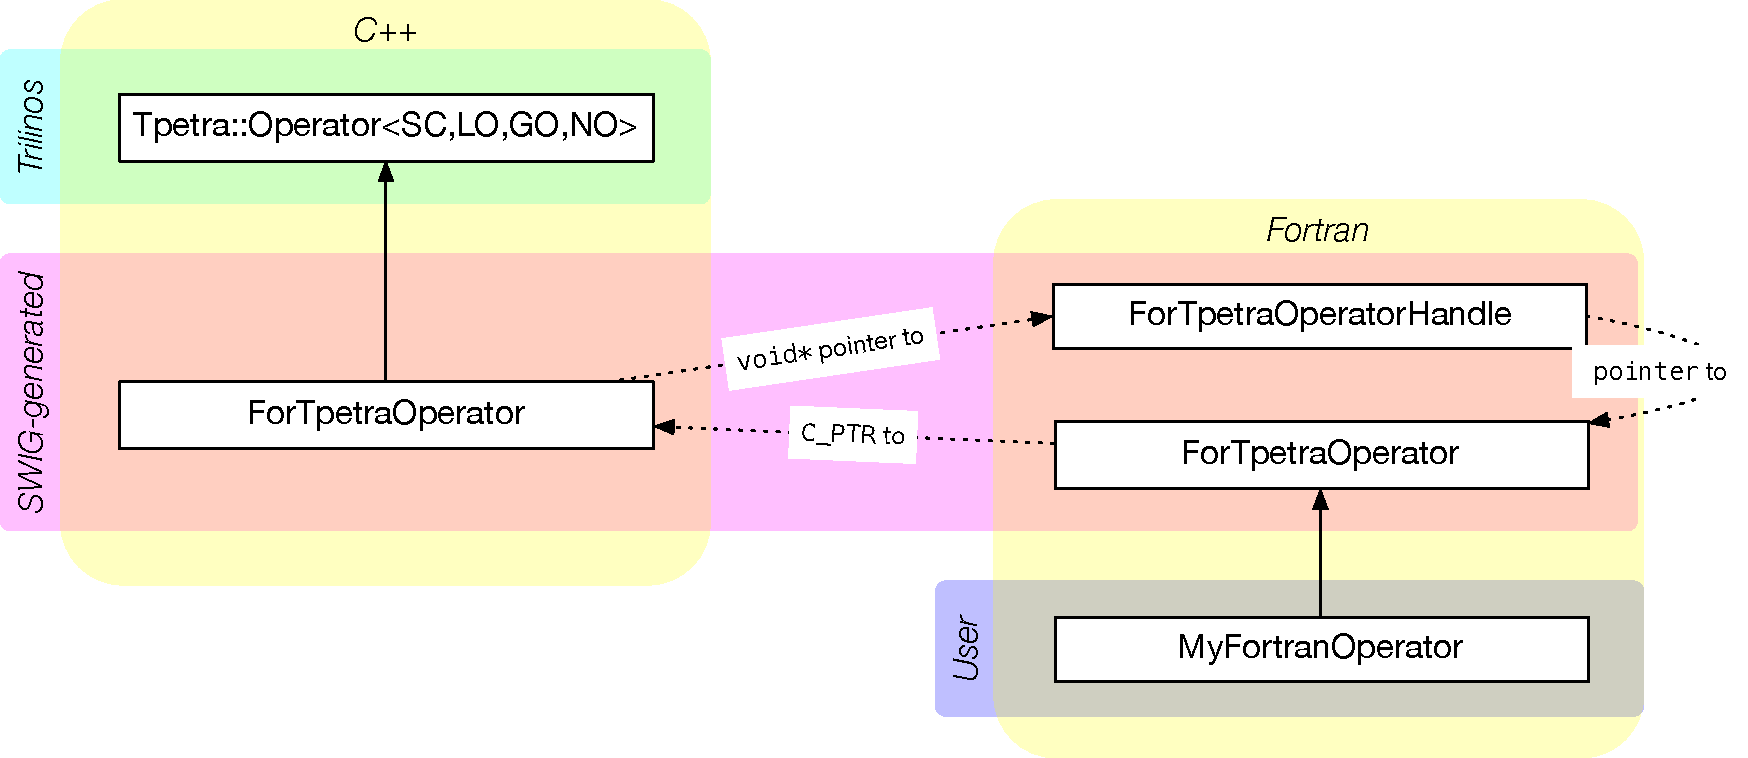
\includegraphics[scale=0.8,width=6in]{projects/2.3.3-MathLibs/2.3.3.14-ALExa-ForTrilinos/ForTrilinos_ioc}
    \caption{\label{fig:fortran_ioc}The proposed Inversion-of-Control approach
    allowing Fortran applications to define operators on Fortran side while
    still using ForTrilinos types.}
\end{figure}

This approach allows the user callback functions to interact with native Fortran
types and ForTrilinos class wrapper types. In the same vein, users would not
have to manually pass \texttt{type(C\_PTR)} instances into and out of the
callback function, as the C++ Fortran conversions can be tedious and
error-prone, which indeed is the motivation for using SWIG to generate
ForTrilinos.  Another important feature is that it allows the application code
to extend Trilinos without having to generate any new interface code, either by
hand or using SWIG. In other words, the Fortran end user should not have to know
C++ or SWIG.

\paragraph{Next Steps}

Our next efforts include:
\begin{enumerate}
  \item \textbf{Provide wrappers for more libraries:} ForTrilinos will continue
    efforts to increase the number of wrapped Trilinos libraries. The scheduled
    release of the next phase of the project will include libraries
    corresponding to nonlinear solvers, such as NOX.
  \item \textbf{Integrate developed capabilities into applications:} E3SM-MMF
    is an Earth system model development and simulation project. It relies on
    Trilinos for its implicit capabilities. The ForTrilinos project will
    integrate the developed nonlinear solver with IoC into E3SM-MMF to provide
    path forward to heterogeneous stack.
  \item \textbf{Provide interfaces for heterogeneous platforms:} ForTrilinos
    will develop support for heterogeneous memory through providing access to
    Kokkos-based interfaces in Trilinos. This will allow full exposure to
    Trilinos capabilities targeting Exascale machines.
\end{enumerate}
